%% Latex instantiation based on template for PhD dissertation or MS thesis
%% Brigham Young University

\documentclass[12pt]{report}

%%%%%%%%%%%%%%%%%%%%%%%%%%%%%%%%%%%%%%%%%%%%%%%%%%%%%%%%
%  Setup BYU thesis format
%%%%%%%%%%%%%%%%%%%%%%%%%%%%%%%%%%%%%%%%%%%%%%%%%%%%%%%%%
\usepackage{csquotes} % This was added by Michael Bean

\usepackage{byustyle}
% Setup the byu style sheet
\byustylesetup{
    %
    %isdissertation = true,            % Uncomment this if you're doing a PhD dissertation
    %etdsubmission = true,            % Uncomment this if you're compiling it for ETD submission
    singlepageabstract = true, % Comment this out if your abstract is multiple pages
    %singlepageacknowledgements = true, % Uncomment this if your Acknowledgements is multiple pages
    %
    % Definitions of names needed in thesis/dissertation
    deptname          = Department of Humanities,    %
    collegename       = Linguistics, %
    committeechairman = Deryle Lonsdale,                      %
    committeemembera  = Mark Davies,                         %
    committeememberb  = Stephen Liddle,                          %
    %committeememberc  = Firstname Mi. Lastname,                    % PhD Only
    %committeememberd  = Firstname Mi. Lastname,                     % PhD Only
    graddate = June 2016,  % Leave commented for current month and year
    %copyrightyear = 2016,      % Leave commented for current year
    % uncomment the keywords for a dissertation
    keywords         = {LDA, Gibbs Sampling, k-NN, Hellinger Distance, Jenson Shannon Divergence, IR, recommendation systems, text mining, LDS Scripture Citation Index, SCI, \emph{RelRec}, topic modeling}
    %
    % Uncomment to shorten for proofreading purposes
    %noabstract = true,         % Don't show the abstract page
    %nouniversitypages = true,  % Don't show any of the "university pages"
    %noacknowledgements = true, % Don't show the Acknowledgements page
    %notableofcontents = true,  % Don't show the Table of Contents
    %nolistoffigures = true,    % Don't show the List of Figures
    %nolistoftables = true,     % Don't show the List of Tables
    notocandlists = true,      % Don't show the Table of Contents, List of Figures, or the List of Tables
    noheaderatall = true,      % Don't show any of the BYU Thesis header pages
}
%%%%%%%%%%%%%%%%%%%%%%%%%%%%%%%%%%%%%%%%%%%%%%%%%%%%%%%%
%  END:  Setup BYU thesis format
%%%%%%%%%%%%%%%%%%%%%%%%%%%%%%%%%%%%%%%%%%%%%%%%%%%%%%%%%

%%%%%%%%%%%%%%%%%%%%%%%%%%%%%%%%%%%%%%%%%%%%%%%%%%%%%%%%
%  Include other \usepackage{} statements here.
%    Add one package at a time.
%    Warning:  Some packages are not compatible with byuthesis.sty
%%%%%%%%%%%%%%%%%%%%%%%%%%%%%%%%%%%%%%%%%%%%%%%%%%%%%%%%%
%\usepackage[normalmargins]{savetrees} % prints smaller to save trees (draft only)
\usepackage{amsmath,amssymb} % math definitions
\usepackage{graphicx}        % for figures
\usepackage{subfigure}       % for figures with multiple subfigures
\usepackage{setspace}        % so all the captions will be single spaced
\usepackage[round,colon]{natbib}
%%%%%%%%%%%%%%%%%%%%%%%%%%%%%%%%%%%%%%%%%%%%%%%%%%%%%%%%
%  END: Include other \usepackage{} statements here.
%%%%%%%%%%%%%%%%%%%%%%%%%%%%%%%%%%%%%%%%%%%%%%%%%%%%%%%%%

%%%%%%%%%%%%%%%%%%%%%%%%%%%%%%%%%%%%%%%%%%%%%%%%%%%%%%%%
% For doing bookmarks in the PDF file
%%%%%%%%%%%%%%%%%%%%%%%%%%%%%%%%%%%%%%%%%%%%%%%%%%%%%%%%%
% For more info, see:
% http://www.geocities.com/kijoo2000/latex2pdf.pdf
% http://www.tug.org/applications/hyperref/manual.html
\usepackage[backref,pagebackref,hidelinks,plainpages=false,driverfallback=dvipdfm]{hyperref}
\hypersetup{
    %bookmarks    = true, % Make bookmarks (default=true). This option
                          %cannot be used after package has been loaded,
                          %thus use like this: \usepackage[bookmarks=false]{hyperref}.
    %
    breaklinks   = false, % Allow link text to break across lines (default=false).
    linktocpage  = false, % make page number, not text, be link on TOC, LOF and LOT
    colorlinks   = false, % Color the text of links (true) or put color frames over
                          % the links (false).
% NOTE: if you need to use a dvi->ps->pdf path for things like PSTricks, you
% may find that commenting out the next line is necessary.
    %pdfborder    = 001,   % sets the default for pdf links
    pdfstartview = {FitH}, % Set the startup page view. Possible options are:
                           % FitH: Fit whole width of page
                           % FitV: Fit whole height of page
                           % FitB: Fit whole Bounding Box page
                           % FitBH: Fit whole width of Bounding Box of page
                           % FitBV: Fit whole height of Bounding Box of page
    bookmarksnumbered  = true, % Put section numbers in bookmarks (default=false)
    bookmarksopen      = true, % Open up the bookmark trees (default=false).
    bookmarksopenlevel = 1, % Level to which bookmarks are open (default=\maxdimen).
    bookmarkstype      = toc, % Specify which toc file to mimic (default=toc).
    pdfpagemode        = {UseOutlines}, %  Specify how document starts when opened ({None}).
                                        % Possible options are:,
                                        % None: Neither bookmarks nor thumbnails are visible.
                                        % UseOutlines: Bookmarks are visible.
                                        % UseThumbs: Thumbnails are visible.
                                        % FullScreen: Full-screen mode
    pdftitle    = {Master's Thesis},
    pdfauthor   = {Michael G. Bean},
    pdfcreator  = {Michael G. Bean},
    pdfsubject  = {Michael G. Bean's Master's Thesis},
    pdfkeywords = {Thesis Template, BYU},
}
%%%%%%%%%%%%%%%%%%%%%%%%%%%%%%%%%%%%%%%%%%%%%%%%%%%%%%%%
%  END: For doing bookmarks in the PDF file
%%%%%%%%%%%%%%%%%%%%%%%%%%%%%%%%%%%%%%%%%%%%%%%%%%%%%%%%%

%%%%%%%%%%%%%%%%%%%%%%%%%%%%%%%%%%%%%%%%%%%%%%%%%%%%%%%%
%                Macros
%  Define macros here
%%%%%%%%%%%%%%%%%%%%%%%%%%%%%%%%%%%%%%%%%%%%%%%%%%%%%%%%%
\def\proof{\noindent{\it Proof: }}
\def\QED{\mbox{\rule[0pt]{1.5ex}{1.5ex}}}
\def\endproof{\hspace*{\fill}~\QED\par\endtrivlist\unskip}
%
\newcommand{\norm}[1]{\left\|#1\right\|}
\newcommand{\abs}[1]{\left|#1\right|}
\newcommand{\defeq}{\stackrel{\triangle}{=}}
\newcommand{\re}{\mathbb{R}} % real numbers
\newcommand{\OMIT}[1]{{}} % omit sections of text
\newcommand{\pd}[2]{\ensuremath{\frac{\partial #1}{\partial #2}}} % partial derivative

%%%%%%%%%%%%%%%%%%%%%%%%%%%%%%%%%%%%%%%%%%%%%%%%%%%%%%%%%
%                End Macros
%%%%%%%%%%%%%%%%%%%%%%%%%%%%%%%%%%%%%%%%%%%%%%%%%%%%%%%%%

% To only print a few chapters without changing the reference numbers,
% uncomment the chapters you want
%\includeonly{chapter_intro}
%\includeonly{chapter_methods}
%\includeonly{chapter_results}
%\includeonly{chapter_conclusion}
%\includeonly{chapter_future_work}
%\includeonly{appendixa}

%%%%%%%%%%%%%%%%%%%%%%%%%%%%%%%%%%%%%%%%%%%%%%%%%%%%%%%%%
% Start Document
%%%%%%%%%%%%%%%%%%%%%%%%%%%%%%%%%%%%%%%%%%%%%%%%%%%%%%%%%

\begin{document}

% Define Title & Author
%\title{\emph{RelRec}, A Textual Recommendation System Optimized for LDS SCI}
\title{Comparing Recommender Systems for Use by the LDS Scripture Citation Index}
\author{Michael G. Bean}

% For displaying the BYU Thesis header
% This command assumes that there are documents called abstract.tex and
% acknowledgements.tex that will be included in the header
\showBYUHeader


% Include chapters of the thesis here:
% each chapter should be in a file with a .tex extension and the text
% of the file should begin with \chapter{Chapter Title}, followed
% by the text of the chapter.
%  Note: the introduction is considered Chapter 1.
%\chapter{Introduction}

In this thesis I address the subject of recommender systems for large textual datasets. Specifically I will be working with the Corpus of LDS General Conference talks (\textit{CLDSGCT}). This dataset grows at least bi-yearly and presently contains over 10k documents. It is frequently accessed because members of the LDS church are asked to use it as a source of personal study and as they teach in their lay church. Therefore it is important that users are able to locate documents that have meaningful connections.

Information retrieval within large sets of textual data such as the \textit{CLDSGCT} is a common problem. Two main approaches to this problem are search and recommendation. Search is when the user enters a text based query and the computer retrieves documents based on that query. An example of this is google search. The weakness with search-based approaches is that it relies on the user to already have an idea of what is within the dataset (i.e. vocabulary) and determine the best search query to access the desired information. The goal of a recommender system is to generate meaningful recommendations to a collection of users for items or products that might interest them. Suggestions for books on Amazon, or movies on Netflix, are real-world examples of the operation of industry strength recommender systems. ``The design of such recommendation engines depends on the domain and the particular characteristics of the data available'' \citep{Melville2010}. These systems have limitations and biases based on the specific recommending algorithms chosen, available data, and domain. Currently users wishing to use the documents found in the \textit{CLDSGCT} can use two websites to help them: \url{LDS.org} and \url{scriptures.byu.edu}. At \url{LDS.org} users can perform a search or browse by topic within a year. At \url{scriptures.byu.edu} users can search for talks by using the parameters of year, speaker, and user query.

I believe the user experience would be improved by a recommender system which, given some starting document, can recommend related documents. The purpose of this thesis is to compare two ways of building a recommender system. They are compared using the catalog coverage metric. Ultimately, the system we select for our use, which has the best catalog coverage, we call RelRec. By using LDA, RelRec automatically identifies latent topics in talks and uses topics to locate similar talks.

%\chapter{Literature Review}

%\chapter{Methodology} \label{chp:chapter2}

\section{Overview}
Docker has quickly become that. This thesis is one evidenced of its growing popularity. % TODO: Move to methodology section.

TODO: Mention why only catalog coverage is used.

I combined the methods used by \citeyearpar{hall-jurafsky-manning:2008:EMNLP} %Hall et al. (2008)
and \citeyearpar{Krstovski2013efficient} %Krstovski (2013)
to the \emph{CLDSGCT}. I then compared performance to that of an \emph{TF-IDF} model using some of the metrics outlined by \citeyearpar{Ge:2010:BAE:1864708.1864761} %Ge et al. (2010)
along with an \emph{nDCG} similarity measure. This involves comparing an LDA-based recommendation system to an off-the-shelf \emph{TF-IDF} recommendation system. Both systems will be parameterized such that they provide the top 5 recommendations for each document. I will use Collapsed Gibbs Sampling to induce parameters for an LDA (topic) model, then feed this output into a k-NN algorithm (k = 5). For k-NN’s distance metric, I will use Hellinger distance. The 5 nearest neighbors will then be sorted from nearest neighbor to farthest. This is the output that will be compared to the top 5 results for each document \emph{TF-IDF} system.

The dataset contains the same documents as those used by Mark Davies in his Corpus of LDS General Conference talks available at http://corpus.byu.edu/gc/. The authorship dates for these talks are ranges of either 1846-1886 or 1942-2013. They total over 1400 talks. Some were extemporaneously given while others were scripted. The intended audience is generally only either the male members of the church, female members of the church, or the entire church. The size and the extent of internationality of the audience is increasing over time. The LDS church currently has over 15 million members, with the majority outside the United States.

To measure the performance of \emph{RelRec}, I performed the following key tasks.

\begin{enumerate}
	\item Use \textit{Collapsed Gibbs Sampling} to infer the parameters of an LDA model;
	\item Use the Mallet toolkit will be used to run collapsed Gibbs sampling;
	\item Use k-NN with the Hellinger distance as the distance metric for \emph{RelRec}; and
	\item Use nDCG to measure similarity with a \emph{TF-IDF} system catalog coverage.
\end{enumerate}

\section{Reproducibility}
In order to be able to reproduce, share, and track work performed in the process of completing this thesis, I versioned code using git. I employed the use of both cutting edge tools as well as well-established ones. The result is code that is both highly capable and easy to follow. Ultimately, I aimed to make the code highly configurable, re-runable, measurable, and shareable.

In this section, methodology will be described, starting with code management \& organization, then tools used (programming languages, CLI tools, operating systems, libraries, databases), followed by models, algorithms \& metrics, concluding with metrics. In Figure \ref{fig:entire_process}, the steps (or modules) of the experiment are shown.

\begin{figure}[hhhhhtb]
	\centering
		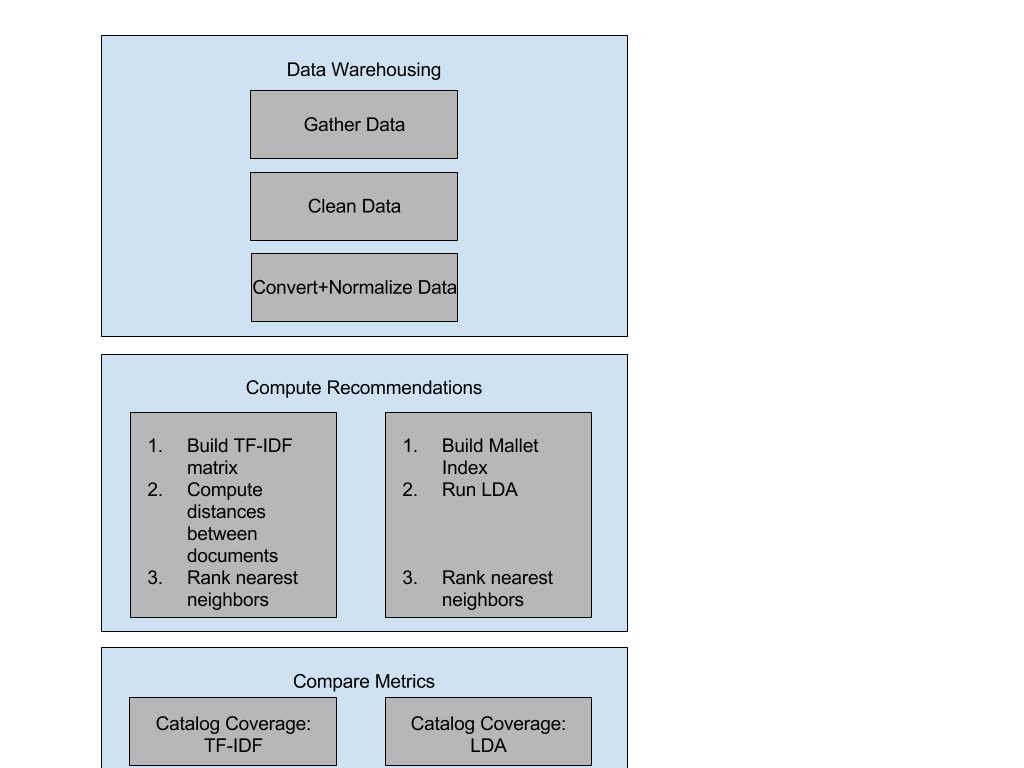
\includegraphics[width=7.5in,natwidth=810,natheight=942]{figures/entire_process.png}
		\caption[Entire Process]{
			Experiment Process\\
			The entire process for the thesis experiment outlined as `modules'. When modules are horizontally adjacent, they may be done in parallel. Note that further parallelization is possible, but not shown. Modules that are higher on the diagram are performed before lower ones.
		}
	\label{fig:entire_process}
\end{figure}

\section{Code Management + Organization}
For the experiment to be robust, it is important that it can be replicated and compared. One of the best ways to allow for this is to make the code both configurable and sharable. Thus, this section is included.

I versioned the experiment’s code in a git project along with data during the gathering process. Whenever a step completes, it outputs data which can be used as input to other modules. The code is modularized such that each docker target corresponds with a module shown previously. The docker daemon builds each target open request (as directed by make), and using docker-compose, directories are connected to the image as volumes. This allows the image to be both modular and systematic. Each docker target has a corresponding file called Dockerfile. Each Dockerfile instructs the docker daemon to obtain requisite packages, e.g. nodeJS, for the module to run the code specific to it. When the code is complete, the docker container terminates, and the next may run when Make instructs it to do so.

Viewing each docker container as a module lends to be seen as a part of the algorithm. Naturally, to each container I map an input and output folder, both located at the root of the file system. The output of multiple containers can be combined as input to subsequent ones, which was sometimes the case here. The first module’s input was actually the database graciously provided by Dr. Steven Liddle, containing pre-downloaded documents to jump-start the project.

I named each docker target logically so upon querying the docker daemon for the list of images, each image would be easy to re-run:

\begin{enumerate}
  \item obtain\_data
  \item compute\_tf\_idf\_recommendations
  \item compute\_lda\_recommendations
  \item etc.
\end{enumerate}

\subsection{Tools, Libraries, OS, Database}
I used various tools in the process of carrying for the preparation and execution of this thesis’ experiment. Table A.1 in the appendix details what they are and what they were used to do.

Core to this project was the use docker. Choosing to use docker forced me to code in all dependencies of each module either as code in the module, or as packages to be installed to each individual docker container during the docker build process. Indeed, the docker daemon builds containers by following instructions given in the files called Dockerfile. This makes each step of the experiment self-documenting. Another benefit of this is that it makes the code cloud-deployable, making it possible to easily offload work to the cloud when appropriate. Offloading to the cloud was not necessary here since I had sufficient computing resources for the project already purchased.

\subsection{Models, Algorithms \& Metrics}
Choice of algorithm \& metrics go hand-in-hand. In fact, algorithm and data can often influence each other, further influencing the selection of metrics. For example, if I were to have a gold standard or baseline of recommendation engines for the 5000+ documents used in this project, I would be able to use nDCG as a metric. Since I do not have such a baseline, such a metric cannot be used. Per xyz, I use catalog coverage, allowing the comparison of two non-baseline algorithms.

Choosing the algorithms for this project was not difficult. I selected \emph{TF-IDF}+kNN and LDA+kNN as my main topic-modeling algorithms. \emph{TF-IDF} is straight-forward to understand and code. LDA is more difficult to code and is actually a topic model. Luckily, open-source projects exist where an algorithm is already provided, which I quickly opted to use.

Given that I had prior experience using Gibbs Sampling to generate LDA models \citep{bean5-LDA-ToT} the choice to select that algorithm was logistical (optimizing to permit me more time to focus on other areas of this work). EM lends itself to parallelization, but on my dataset, I knew that Gibbs Sampling would only take about 10 minutes to run, which is not an issue. The cost-benefit of changing algorithms was too high, at least when it comes to building the LDA model via parallelized algorithm. In my case, I used the mallet toolbox \citep{McCallumMALLET} (TODO: cite previously) which provides the Gibbs Sampling algorithm to infer parameters of the the LDA model.

% TODO: Double check whether Jenson-Shannon was used (check prospectus).
% TODO: Add more algorithm notes here and move this table to a better location.
% TODO: 'core module' is a new term introduced here!
\begin{center}
	\begin{tabular}[pos]{| l | l | l | l | l | l |}
		\hline
		Algorithm & Variable Name & Variable Type & Input Value & Use & Reason \\ \hline

		k-NN & k & integer & 100 & Sets number of neighbors to \\ return for each document. & Using a value of 100 requires more computing, but also allows us to compare the models for up to 100 recommendations per document. \\ \hline

		Gibbs Sampling & t & integer & 250 & Sets number of topics to find & In previous research I determined that 250 was a good number for this variable. \\ \hline

		k-NN distance metric \\
		for \emph{TF-IDF} model & distance & function & Cosine & Distance metric allows algorithm to measure distance between documents in the model. & Intuitive and well-known. Others functions exist for this, but are left to future work to use. \\ \hline

		k-NN distance metric \\
		for LDA model & distance & function & Jenson-Shannon & Distance metric allows algorithm to measure distance between documents in the model. & Well-known and works for vectors in the probability simplex. \\ \hline

		\emph{TF-IDF} & stop words & list of word strings & none & Sets words to ignore in model. & Assigns words a value of 0 TF and 0 IDF values or removes them altogether to shrink vector space and accelerate computing (depends on actual algorithm implementation). \emph{TF-IDF} is robust against high-frequency words since they automatically receive low TF and low IDF values. \\ \hline

		Preparing input LDA & stop words & list of word strings & default mallet list + handful of religious words [TODO: which words?] & Removes stopwords at indexing time (module x [TODO: name exact module here]). & LDA is not super robust against common words. \\ \hline
		normalization & to\_lower\_case & boolean & true & If true, tells algorithm to lowercase all text. & To allow all following algorithms to ignore case, the simplest way to do so was to lowercase everything before completing the data preparation core module. \\ \hline
	\end{tabular}
\end{center}

% TODO: \cite instead of link?
The core of this project came down to organization, good testing (to ensure bug-free code), and study of any tools that would end up being helpful in processing. kNN is a machine learning algorithm which as input requires the value for k and a selection of a distance metric. The output of \emph{TF-IDF} and LDA are both in vectors, but LDA’s vectors lay within the probability simplex. Distance metrics had to be appropriate for the space. For \emph{TF-IDF} vectors, I opted to use cosine similarity; for LDA, Jensen-Shannon (\url{https://en.wikipedia.org/wiki/Jensen%E2%80%93Shannon_divergence, http://maroo.cs.umass.edu/pub/web/getpdf.php?id=1101}). % TODO: (or was it Hellinger? \url{https://www.quora.com/How-can-I-compute-the-Hellinger-distance-between-documents-based-on-topic-proportions-generated-by-Latent-Dirichlet-Allocation}).

To evaluate the recommendations provided as output from the ordered kNN results, a common metric had to be employed. I chose to measure the goodness of each set using the catalog coverage metric. % TODO: remove passive voice here.

For reproducibility, the following table shows the values, settings, and configurations selected for the algorithms.

By using the aforementioned metrics, this study aims to prove the following hypothesis
	\begin{quote}
		$H_{1}:$ \emph{RelRec} will provide better coverage than a \emph{TF-IDF} system.

		%$H_{2}:$ \emph{RelRec} is more intuitive than emph recommendation systems since it has greater ability to disambiguate word sense by topic.
	\end{quote}

%\chapter{Results \& Evaluation} \label{chp:chapter3}

[TODO: insert here: samples of topics: a sanity check]

[TODO: insert here: samples of \emph{TF-IDF} words]

[TODO: insert here: display graph of results]

\begin{figure}[hhhhhtb]
	\centering
		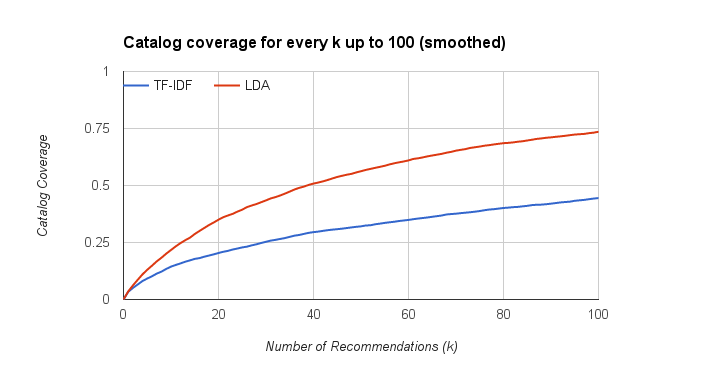
\includegraphics[width=5.5in,natwidth=510,natheight=642]{figures/catalog_coverage_0_100.png}
		\caption[Catalog Coverage Values for All Models]{
			Catalog Coverage Values for All Models
		}
	\label{fig:catalog_coverage_0_100}
\end{figure}

[TODO: insert here: display some topics here, put full list of topics in appendix?]

\chapter{Conclusion} \label{chp:chapter4}

In our case, we wanted to have a good catalog coverage, but have intuitive results as well. Both \emph{TF-IDF} and LDA could provide intuitive results, but LDA provides the best catalog coverage when showing the top 5 results for each document.

%[TODO: Move this to its own chapter?]

\section{Future Work}
The experiment described here lends itself to future work. It can be easily adapted to use a different set of documents as input. Furthermore, settings may be easily modified to change the number of topics discovered for the LDA topic model, stop word lists, normalization functions, and distance metrics. In particular, an area where this might be particularly interesting and perhaps novel would be to do this on chapters of scripture. Indeed, for those who wish to locate chapters of related content between works of differing religions, one would only need to provide the engine I used here with all chapters from each work as separate documents (e.g. Bible vs. Qur'an, Bible vs. Book of Mormon vs. Doctrine and Covenants, etc.). Perhaps the most interesting combination for the LDS church as a whole would be to perform this on the Bible, the Book of Mormon, the Doctrine and Covenants, and the Pearl of Great Price as input, the model could be used to enhance current LDS scriptural footnotes.





%%%%%%%%%%%%% begin Bibliography %%%%%%%%%%%%%%%%%
%\phantomsection %Forces a new section prior to setting the bibliography reference point
\addcontentsline{toc}{chapter}{Bibliography}
\bibliographystyle{plainnat}
\bibliography{refs}

% Bibliographies are best created and maintained using BibTeX
% To use Bibtex, create a bibliography file, e.g., refs.bib
% The sample file sources.bib shows examples of different
% bibliographic entries.
% The bibliography is created by executing:
%  1.  latex, 2. bibtex, 3. latex, 4. latex
%%%%%%%%%%%%%%%% end Bibliography %%%%%%%%%%%%%%%%%

%Included because WinEdit is RETARDED and it needs it for Gather Purposes:
%input "refs.bib"


% Include appendix sections here:
% each appendix should be a file with a .tex extension and the text
% of the file should begin with \appendix{Appendix Title}, followed
% by the contents of the appendix
%\appendix{Sample Appendix}

\section{Width Based on Page Size Figure Example} \label{sec:appendxia_figure_example}
Here's an example of a figure whose width depends on the width
of the page. You can see if as Figure \ref{fig:appendix_some_pic}.

\begin{figure}[htbp]
  \centering
  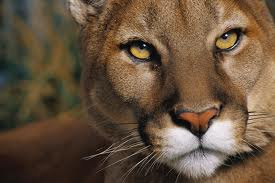
\includegraphics[width=0.45\textwidth]{figures/appendixa/some_pic}
  \caption[Example Width Based on Page Size Figure]{
    This is an example of a figure whose width will be 45\% of the
    width of the page. If you'd like to see a figure with a fixed
    width then you can see it as Figure \ref{fig:intro_stuff} in
    Section \ref{sec:intro_figure_example}. Just FYI, I made this
    figure with PowerPoint and then copied it and pasted it into
    wmf2eps and choose the "Paste EMF" option. It will generate
    a larger file, but it will look a TON better than the
    "Paste WMF" option and the "Paste DIB" option will paste the
    rasterized image that won't scale well at all.}
  \label{fig:appendix_some_pic}
\end{figure}
%\appendix{Tools \& Links}
\label{tools+links}

\section{Open-Source Tools: Docker, Mallet, npm}

\subsection{Docker*}
Now that algorithms and metrics have been discussed, we can move on to discussing tools that can be used to create reproducible, robust, systems.

%Core to this project is the use of docker.
Dockers are Linux containers which the docker-engine (i.e. docker daemon) can build and run. They can be thought of as Linux virtual machines in some ways, although they tend to be resource/hardware agnostic since they simply share the kernel, RAM, and other hardware on the host on which they are run. They are considered lightweight since instead of running the full Linux stack for each container, only necessary files are run from within the container. This has made it easy for a new market to emerge where products that are software as a service (SaaS) can be hosted at a lower cost. Container Engine by Google (\url{https://cloud.google.com/container-engine/}) and tutum by Tutum (\url{https://www.tutum.co/}) are examples of this.

Docker has a growing community around it. In fact, Google has created an open-source project called Kubernetes which aims to ``accelerate Dev and simplify Ops'' \citep{kube_website}. According to \citet{google_container_engine}, it is used under the covers for Container Engine, a Google cloud product. Although Linux containers have been around for some time now, the docker community has made it much more mainstream, especially for computing environments where scaling horizontally is important. Thus, companies such as Netflix and EMC find it highly beneficial. In the authors experience, Linux tools with growing communities are well backed, become robust, and tend to be both easy to use as well as empowering.

\subsection{Mallet Toolbox}
Mallet toolbox

\subsection{Node Package Manager (NPM)}
 \url{https://www.npmjs.com/}

% Consider not using comma-delimiting
\begin{center}
	\begin{tabular}[pos]{| l | l | l |}
		\hline
		Tool/Library & Use & Link \\ \hline
		git & code versioning; code sharing & \url{https://git-scm.com/about} \\ \hline
		Latex, Google Docs, Microsoft Office & Composing this document & \url{https://www.latex-project.org/}, \url{https://docs.google.com}, \url{https://products.office.com/en-us/word} \\ \hline
		AntConc & Indexing of files to locate high-frequency words later used as stop words. & \url{http://www.laurenceanthony.net/software/antconc/} \\ \hline
		``docker'' (docker daemon, docker-compose, docker containers) & Containerization and modularization of each module such that when running, code for each module only contains input, the necessary code, output, and operating system tools. & \url{https://www.docker.com/} \\ \hline
		mysql SCI database & Input into first module & \url{link not available} \\ \hline
		mysql server, mysql client & hosting + querying of SCI database & \url{http://dev.mysql.com/} \\ \hline
		GNUMake & orchestration of modules (i.e. the command ‘make thesis’ runs each module that hasn’t been run, making sure to do so in the correct order & \url{https://www.gnu.org/software/make/} \\ \hline
		nodeJS, sh, bash, zsh & orchestration of modules (i.e. the command ‘make thesis’ runs each module that hasn’t been run, making sure to do so in the correct order & \url{https://nodejs.org/en/}, \url{https://www.gnu.org/software/bash/} \\ \hline
		VirtualBox & running docker daemon via boot2docker (Linux VM) & \url{https://www.virtualbox.org/} \\ \hline
		Atom, vi, nano & code editors & \url{https://atom.io/}, \url{http://www.vim.org/}, \url{http://www.nano-editor.org/} \\ \hline
		mallet & indexing of files in preparation for LDA; Gibbs Sampling to infer parameters of LDA topic model & \url{http://mallet.cs.umass.edu/} \\ \hline
		Mac OS-X & Host system running VM, hosting code & \url{http://www.apple.com/osx/} \\ \hline
		Bitbucket & code hosting & \url{https://bitbucket.org/} \\ \hline
		GitHub & code hosting location of open-source tools used in the project including nodeJS and mallet & \url{https://github.com/} \\ \hline
		less, more, cat, wc,  grep, egrep, z, oh-my-zsh & general modification or searching of files in *nix & \url{https://en.wikipedia.org/wiki/Less_(Unix)}, \url{http://linux.die.net/man/1/more}, \url{http://linux.die.net/man/1/grep}, \url{http://linux.die.net/man/1/egrep}, \url{http://linux.die.net/man/1/wc}, \url{https://github.com/rupa/z}, \url{https://github.com/robbyrussell/oh-my-zsh} \\ \hline
		regular expressions & easy removal of boiler plate HTML from documents & \url{https://en.wikipedia.org/wiki/Regular_expression} \\ \hline
		npm & hosting of open-source code used in nodeJS & \url{https://www.npmjs.com/} \\ \hline
		\hline
	\end{tabular}
\end{center}


%End the document
\end{document}
